\documentclass[11pt,a4paper]{article}

\usepackage[margin=0.5in, top=3cm, bottom=2cm]{geometry}
\usepackage[spanish, activeacute]{babel}
\usepackage[utf8]{inputenc}
\usepackage{amsthm}
\usepackage{amsmath}
\usepackage{amsfonts}
\usepackage{amssymb}
\usepackage{graphicx} %Para incluir el logo de la UBA
\usepackage{caratula} %Para armar el cuadro de integrantes
\usepackage{todonotes}
\usepackage{float}
\usepackage[lined,ruled,linesnumbered]{algorithm2e}
\usepackage{hyperref}
\usepackage{xcolor}
\usepackage[final]{pdfpages}
\providecommand{\DontPrintSemicolon}{\dontprintsemicolon}

\graphicspath{{imagenes/}}

\newcommand\comentario[2]{\textbf{{[#1: \textcolor{red}{#2}}}]}
\renewcommand\comentario[2]{}

\setcounter{secnumdepth}{5}

\begin{document}

\integrante{Maurizio, Miguel Sebasti\'{a}n}{635/11}{miguelmaurizio.92@gmail.com}
\integrante{Prillo, Sebasti\'{a}n}{616/11}{sebastianprillo@gmail.com}
\integrante{Tagliavini Ponce, Guido}{783/11}{guido.tag@gmail.com}

\def\Materia{Bases de Datos}
\def\Titulo{Trabajo Pr\'{a}ctico 2}
\def\Fecha{10 de noviembre de 2015}

%----- CARATULA -----%

\thispagestyle{empty}

\begin{center}
	
\includegraphics[scale = 0.25]{imagenes/logo_uba.jpg}
\end{center}

\begin{center}
	{\textbf{\large UNIVERSIDAD DE BUENOS AIRES}}\\[1.5em]
	{\textbf{\large Departamento de Computaci\'{o}n}}\\[1.5em]
    {\textbf{\large Facultad de Ciencias Exactas y Naturales}}\\
    \vspace{35mm}
    {\LARGE\textbf{\Materia}}\\[1em]    
    \vspace{15mm}
    {\Large \textbf{\Titulo}}\\[1em]
    \vspace{15mm}
    {\textbf{\Large \Fecha}}\\
    \vspace{15mm}
    \textbf{\tablaints}
\end{center}

\newpage
\thispagestyle{empty}
\tableofcontents

\parskip=5pt
\setlength{\parindent}{0pt}

\newpage
\setcounter{page}{1}
\pagenumbering{arabic}
\pagestyle{plain}

\section{Introducci'on}
\section{Ejercicio 1}

En este ejercicio dise\~namos una base de datos NoSQL de tipo documentos con la capacidad de responder rapidamente a varias consultas. Para ello, empleamos desnormalizaci'on, dise\~nando documentos adecuados para las consultas.

\subsection{Desnormalizaci'on}

Desnormalizamos el esquema, de la forma tradicional. Cada entidad tiene un documento asociado. Las relaciones 1:N se incluyen en el documento asociado al lado 1. Las relaciones N:M se incluyen a ambos lados de la relaci'on.

\subsubsection{Documento \texttt{empleados}}

\begin{verbatim}
empleados {
    nro_legajo : INTEGER
    nombre : STRING
    clientes_atendidos : [{dni : STRING, edad : INTEGER, fecha : DATETIME}]
    sectores_donde_trabaja : [{cod_sector : INTEGER, id_tarea : INTEGER}]
}
\end{verbatim}

Observar que en \texttt{clientes\_atendidos} nos guardamos, adem'as del atributo identificatorio \texttt{dni} y el atributo de relaci'on \texttt{fecha}, la \texttt{edad} de los clientes atendidos. Este atributo ser'a necesario para responder una de las consultas, posteriormente. 

Insertamos algunos documentos:

\begin{verbatim}
db.empleados.insert({
    nro_legajo : 1,
    nombre : "empleado1",
    clientes_atendidos : [	{dni : "11111111", edad : 18, fecha : "01/01/2015"},
                           {dni : "22222222", edad : 17, fecha : "01/02/2015"}],
    sectores_donde_trabaja : [{cod_sector : 1, id_tarea : 1} , 	{cod_sector : 2, cod_tarea : 1}]
})

db.empleados.insert({
    nro_legajo : 2,
    nombre : "empleado2",
    clientes_atendidos : [ {dni : "22222222", edad : 17, fecha : "02/02/2015"} ],
    sectores_donde_trabaja : [{cod_sector : 1, id_tarea : 1}, 	{cod_sector : 2, cod_tarea : 1}]
})

db.empleados.insert({
    nro_legajo : 3,
    nombre : "empleado3",
    clientes_atendidos : [{dni : "33333333", edad : 19, fecha : "01/03/2015"}],
    sectores_donde_trabaja : [{cod_sector : 1, id_tarea : 1}, 	{cod_sector : 2, cod_tarea : 1}]
})

db.empleados.insert({
    nro_legajo : 4,
    nombre : "empleado4",
    clientes_atendidos : [],
    sectores_donde_trabaja : [{cod_sector : 1, id_tarea : 1}]
})
\end{verbatim}

\subsubsection{Documento \texttt{articulos}}

\begin{verbatim}
articulos {
    codigo : STRING
    nombre : STRING
    ventas : [{dni : STRING}]
}
\end{verbatim}

Insertamos algunos documentos:

\begin{verbatim}
db.articulos.insert({
    codigo : "1",
    nombre : "articulo1",
    ventas : [{dni :	 "11111111"}, {dni : "22222222"}]
})

db.articulos.insert({
    codigo : "2",
    nombre : "articulo2",
    ventas : [{dni : "11111111"}, {dni : "33333333"}]
})

db.articulos.insert({
    codigo : "3",
    nombre : "articulo3",
    ventas : [{dni : "33333333"}]
})
\end{verbatim}

\subsubsection{Documento \texttt{sectores}}

\begin{verbatim}
sectores{
    cod_sector : INTEGER
    articulos : [{codigo : STRING}]
    trabaja : [{nro_legajo : INTEGER, id_tarea : INTEGER}]
}
\end{verbatim}

Insertamos algunos documentos:

\begin{verbatim}
db.sectores.insert({
    cod_sector : 1,
    articulos : [{codigo : "1"}],
    trabaja : [	{nro_legajo : 1, id_tarea : 1},
               {nro_legajo : 2, id_tarea : 1},
               {nro_legajo : 3, id_tarea : 1},
               {nro_legajo : 4, id_tarea : 1}]
})

db.sectores.insert({
    cod_sector : 2,
    articulos : [{codigo : "2"}],
    trabaja : [	{nro_legajo : 1, id_tarea : 1},
               {nro_legajo : 2, id_tarea : 1},
               {nro_legajo : 3, id_tarea : 1}]
})
\end{verbatim}

\subsubsection{Documento \texttt{clientes}}

\begin{verbatim}
clientes{
    dni : STRING
    nombre : STRING,
    edad : INTEGER,
    atendido_por : [{nro_legajo : INTEGER, fecha : DATETIME}],
    compro_articulos : [{codigo : INTEGER}]
}
\end{verbatim}

Insertamos algunos documentos:

\begin{verbatim}
db.clientes.insert({
    dni : "11111111",
    nombre : "cliente1",
    edad : 18,
    atendido_por : [{nro_legajo : 1, fecha : "01/01/2015"}],
    compro_articulos : [{codigo : "1"} , {codigo : "2"}]
})

db.clientes.insert({
    dni : "22222222",
    nombre : "cliente2",
    edad : 17,
    atendido_por : [{nro_legajo : 1, fecha : "01/02/2015"} , {nro_legajo : 2, 
                                                              fecha : "02/02/2015"}],
    compro_articulos : [{codigo : "1"}]
})

db.clientes.insert({
    dni : "33333333",
    nombre : "cliente3",
    edad : 19,
    atendido_por : [{nro_legajo : 1, fecha : "01/03/2015"}],
    compro_articulos : [{codigo : "2"} , {codigo : "3"}]
})
\end{verbatim}

\subsubsection{Documento \texttt{tareas}}

Si bien este documento no es estrictamente necesario para poder responder a las consultas, incluimos su definici'on por completitud.

\begin{verbatim}
tareas{
    id_tarea : INT,
    descripcion : STRING,
    empleados_realizandola : [{nro_legajo : INTEGER, cod_sector: INTEGER}]
}
\end{verbatim}

\subsection{Consultas}

\subsubsection{Los empleados que atendieron clientes mayores de edad}

\begin{verbatim}
db.empleados.find(
    {"clientes_atendidos.edad" : {$gte : 18}},
    {nro_legajo : 1, nombre : 1}
)
\end{verbatim}

Equivalenemente, podriamos pedir:

\begin{verbatim}
db.empleados.find(
    {"clientes_atendidos" : {$elemMatch : {"edad" : {$gte : 18}}}},
    {nro_legajo : 1, nombre : 1}
)
\end{verbatim}

La query nos retorna, como deseamos:

\begin{verbatim}
{ "_id" : ObjectId("56420cfd92d300ad159887da"), "nro_legajo" : 1, "nombre" : "empleado1" }
{ "_id" : ObjectId("56420cfd92d300ad159887dc"), "nro_legajo" : 3, "nombre" : "empleado3" }
\end{verbatim}

\subsubsection{Los art'iculos m'as vendidos}

\begin{verbatim}
db.articulos.aggregate([
    {$project : {"cant_ventas" : {$size : "$ventas"} , nombre : 1, codigo : 1}},
    {$sort : {"cant_ventas" : -1}},
])
\end{verbatim}

La respuesta a esta consulta es:

\begin{verbatim}
{ "_id" : ObjectId("56420d1e92d300ad159887de"), "codigo" : "1", "nombre" : "articulo1",
    "cant_ventas" : 2 }
{ "_id" : ObjectId("56420d1e92d300ad159887df"), "codigo" : "2", "nombre" : "articulo2",
    "cant_ventas" : 2 }
{ "_id" : ObjectId("56420d1e92d300ad159887e0"), "codigo" : "3", "nombre" : "articulo3",
    "cant_ventas" : 1 }
\end{verbatim}

As'i, vemos que los articulos mas vendidos son los de codigo 1 y 2, cada uno con 2 ventas.


\subsubsection{Los sectores donde trabajan exactamente 3 empleados}

\begin{verbatim}
db.sectores.find(
    {trabaja : {$size : 3}},
    {cod_sector : 1}
)
\end{verbatim}

La respuesta a esta consulta es:

\begin{verbatim}
{ "_id" : ObjectId("56420d9e92d300ad159887e2"), "cod_sector" : 2 }
\end{verbatim}

Efectivamente, el sector 2 contiene exactamente 3 trabajadores.


\subsubsection{El empleado que trabaja en m'as sectores}

\begin{verbatim}
db.empleados.aggregate([
    {$project : {cant_sectores : {$size : "$sectores_donde_trabaja"} , nombre : 1, nro_legajo : 1}},
    {$sort : {cant_sectores : -1}},
    {$limit : 1}
])
\end{verbatim}

La respuesta a esta consulta es:

\begin{verbatim}
{ "_id" : ObjectId("56420cfd92d300ad159887da"), "nro_legajo" : 1, "nombre" : "empleado1",
    "cant_sectores" : 2 }
\end{verbatim}

Si bien los empleados 2 y 3 tambien trabajan en dos sectores, solo se nos pide dar uno solo, asi que desempatamos arbitrariamente.

\subsubsection{Ranking de los clientes con mayor cantidad de compras}

\begin{verbatim}
db.clientes.aggregate([
    {$project : {cant_compras : {$size : "$compro_articulos"} , nombre : 1, dni : 1}},
    {$sort : {cant_compras : -1}}
])
\end{verbatim}

La respuesta a esta consulta es:

\begin{verbatim}
{ "_id" : ObjectId("56420df292d300ad159887e3"), "dni" : "11111111", "nombre" : "cliente1",
    "cant_compras" : 2 }
{ "_id" : ObjectId("56420df392d300ad159887e5"), "dni" : "33333333", "nombre" : "cliente3",
    "cant_compras" : 2 }
{ "_id" : ObjectId("56420df292d300ad159887e4"), "dni" : "22222222", "nombre" : "cliente2",
    "cant_compras" : 1 }
\end{verbatim}

Como vemos, los clientes aparecen ordenamos de mayor a menos cantidad de compras.

\subsubsection{Cantidad de compras realizadas por clientes de misma edad}

\begin{verbatim}
db.clientes.aggregate([
    {$project : {cant_compras : {$size : "$compro_articulos"} , nombre : 1, dni : 1, edad : 1}},
    {$group :{
        _id : "$edad",
        total_compras : {$sum : "$cant_compras"}
    }}
])
\end{verbatim}

El resultado de la query es:

\begin{verbatim}
{ "_id" : 19, "total_compras" : 2 }
{ "_id" : 17, "total_compras" : 1 }
{ "_id" : 18, "total_compras" : 2 }
\end{verbatim}

En definitiva, este es un diseño de documentos que, mediante documentos adecuados y redundancia, permite responder rapidamente a todas las queries pedidas.

\section{Ejercicio 2}

\subsection{Consultas}

\subsubsection{Cantidad de disposiciones tipo \textit{resoluciones} que se hayan realizado en Abril de 2013}

\begin{verbatim}
var map1 = function(){
    emit(this["Tipo"],1)
}

var reduce1 = function(key,values){
    return Array.sum(values)
}

db.disposiciones.mapReduce(map1,reduce1,{query : {FechaDisposicion : {$regex : /^2013-04-/},
 Tipo : "Resoluciones"}, out : "map_res"})
db.map_res.find()
\end{verbatim}

El resultado de esta consulta es:

\begin{verbatim}
{ "_id" : "Resoluciones", "value" : 642 }
\end{verbatim}

\subsubsection{Cantidad de disposiciones por cada tipo definido}

\begin{verbatim}
var map2 = function(){
    emit(this["Tipo"],1)
}

var reduce2 = function(key,values){
    return Array.sum(values)
}

db.disposiciones.mapReduce(map2,reduce2,{query : {}, out : "map_res"})
db.map_res.find()
\end{verbatim}

El resultado de esta consulta es:

\begin{verbatim}
{ "_id" : "", "value" : 3 }
{ "_id" : "Acuerdos", "value" : 2790 }
{ "_id" : "Acuerdos del Consejo de Gobierno", "value" : 160 }
{ "_id" : "Anuncios", "value" : 17226 }
{ "_id" : "Candidaturas", "value" : 1 }
{ "_id" : "Certificaciones", "value" : 72 }
{ "_id" : "Circular", "value" : 1 }
{ "_id" : "Conflictos Positivos", "value" : 6 }
{ "_id" : "Correcciones de Erratas", "value" : 59 }
{ "_id" : "Correcciones de Errores", "value" : 321 }
{ "_id" : "Correcciones de erratas", "value" : 8 }
{ "_id" : "Correcciones de errores", "value" : 44 }
{ "_id" : "Corrección de errores", "value" : 1 }
{ "_id" : "Correción de errores", "value" : 1 }
{ "_id" : "Cuestiones de Inconstitucionalidad", "value" : 1 }
{ "_id" : "Decretos", "value" : 828 }
{ "_id" : "Decretos Legislativos", "value" : 5 }
{ "_id" : "Decretos del Presidente", "value" : 13 }
{ "_id" : "Decretos-leyes", "value" : 15 }
{ "_id" : "Edictos", "value" : 3223 }
{ "_id" : "Instrucciones", "value" : 2 }
{ "_id" : "Leyes", "value" : 12 }
{ "_id" : "Notificaciones", "value" : 768 }
{ "_id" : "Orden", "value" : 4 }
{ "_id" : "Otros", "value" : 45 }
{ "_id" : "Reales Decretos", "value" : 5 }
{ "_id" : "Recursos de Inconstitucionalidad", "value" : 7 }
{ "_id" : "Requisitorias", "value" : 2 }
{ "_id" : "Resoluciones", "value" : 13956 }
{ "_id" : "Órdenes", "value" : 2061 }
{ "_id" : "Órdenes de Comision Delegada", "value" : 2 }
\end{verbatim}

\subsubsection{Fecha m'as citada para todos los informes}

\begin{verbatim}
var map3 = function(){
    emit(this["FechaBOJA"],1)
}

var reduce3 = function(key,values){
    return Array.sum(values)
}

db.disposiciones.mapReduce(map3,reduce3,{query : {}, out : "map_res"})
db.map_res.find().sort({value : -1}).limit(1)
\end{verbatim}

El resultado de esta consulta es:

\begin{verbatim}
{ "_id" : "01/08/2012", "value" : 242 }
\end{verbatim}

\subsubsection{M'axima cantidad de p'aginas utilizadas por cada tipo de disposici'on}

\begin{verbatim}
var map4 = function(){
    emit(this["Tipo"],this["PaginaFinal"] - this["PaginaInicial"] + 1)
}

var reduce4 = function(key,values){
    res = values[0]
    for (var i=1; i < values.length; i++){
        if(res < values[i]){
            res = values[i]
        }
    }
    return res
}

db.disposiciones.mapReduce(map4,reduce4,{query : {}, out : "map_res"})
db.map_res.find()
\end{verbatim}

El resultado de esta consulta es:

\begin{verbatim}
{ "_id" : "", "value" : 16 }
{ "_id" : "Acuerdos", "value" : 12 }
{ "_id" : "Acuerdos del Consejo de Gobierno", "value" : 83 }
{ "_id" : "Anuncios", "value" : 393 }
{ "_id" : "Candidaturas", "value" : 68 }
{ "_id" : "Certificaciones", "value" : 47 }
{ "_id" : "Circular", "value" : 3 }
{ "_id" : "Conflictos Positivos", "value" : 1 }
{ "_id" : "Correcciones de Erratas", "value" : 174 }
{ "_id" : "Correcciones de Errores", "value" : 99 }
{ "_id" : "Correcciones de erratas", "value" : 10 }
{ "_id" : "Correcciones de errores", "value" : 5 }
{ "_id" : "Corrección de errores", "value" : 1 }
{ "_id" : "Correción de errores", "value" : 1 }
{ "_id" : "Cuestiones de Inconstitucionalidad", "value" : 1 }
{ "_id" : "Decretos", "value" : 492 }
{ "_id" : "Decretos Legislativos", "value" : 37 }
{ "_id" : "Decretos del Presidente", "value" : 3 }
{ "_id" : "Decretos-leyes", "value" : 139 }
{ "_id" : "Edictos", "value" : 48 }
{ "_id" : "Instrucciones", "value" : 3 }
{ "_id" : "Leyes", "value" : 194 }
{ "_id" : "Notificaciones", "value" : 11 }
{ "_id" : "Orden", "value" : 7 }
{ "_id" : "Otros", "value" : 65 }
{ "_id" : "Reales Decretos", "value" : 1 }
{ "_id" : "Recursos de Inconstitucionalidad", "value" : 1 }
{ "_id" : "Requisitorias", "value" : 1 }
{ "_id" : "Resoluciones", "value" : 454 }
{ "_id" : "Órdenes", "value" : 634 }
{ "_id" : "Órdenes de Comision Delegada", "value" : 2 }
\end{verbatim}
\section{Ejercicio 3}

\subsection{Ejemplo de sharding en Mongo}

Seguimos las sugerencias del enunciado y analizamos los efectos de usar sharding simple o hasheado en una base de datos en la que insertamos iterativamente tandas de a 20000 registros, para un total de 25 tandas. A continuaci'on mostramos los gr'aficos de carga de los shards a lo largo de las iteraciones:

\begin{figure}[H]
	\begin{center}
		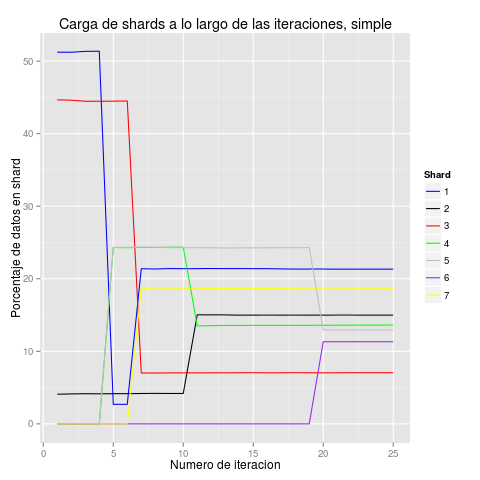
\includegraphics[scale=0.6]{imagenes/siete_shards_simple.png}
	\end{center}
\end{figure}

\begin{figure}[H]
	\begin{center}
		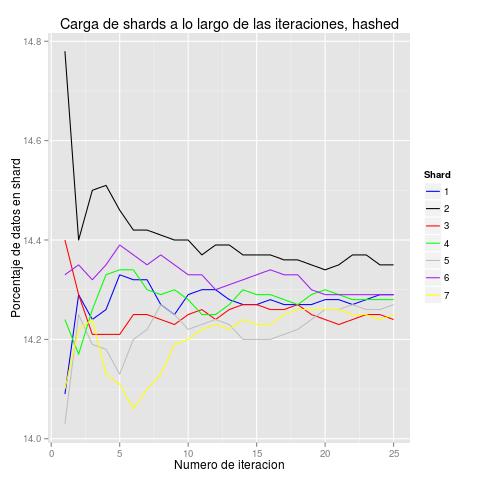
\includegraphics[scale=0.6]{imagenes/siete_shards_hashed.png}
	\end{center}
\end{figure}

Recordemos que el atributo usado de clave para los shards simples es el codigo postal, que es un entero de hasta 6 d'igitos. Cuando se usa un hash para shardear, se lo hace sobre el atributo \_id.

Como podemos apreciar, cuando hacemos sharding hasheando, la distribuci'on de los datos a lo largo de los shards tiende a estar bien balanceada. Por el contrario, si no se usa hash y en cambio se emplea el codigo postal directamente, mongo empieza cargando fuertemente dos shards, y recien despues de un rato empiezan a tener participacion los dem'as shards. Esto se debe a que la forma de determinar qu'e documentos van a qu'e shards cuando se shardea por c'odigo postal se determina en base a interavlos contiguos de esta variable, que mongo no conoce a priori y debe ir estimando. Una vez que la cantidad de datos crece, mongo puede inferir que la distribuci'on del codigo postal es en uniforme entre cero y un millon y la carga se empieza a equilibrar entre los shards. A'un as'i, la carga nunca se empareja tanto como cuando hasheamos.

\subsection{Caracter'isticas de un buen atributo para sharding}

Para que un atributo sea un buen candidato para aplicar la t'ecnica de sharding, debe ser tal que al particionar los datos por ese atributo, las clases que se formen sean de tama\~nos similares. Esto permite que la carga sobre los shards est'e bien distribu'ida, no s'olo en t'erminos del vol'umen de cada shard, sino tambi'en en el sentido de que los accesos y escrituras sean uniformes. Bajo estas condiciones obtendremos una mejor performance de I/O. Espec'ificamente, la latencia y el tiempo de respuesta de los mismos ser'an bajos, gracias a que evitamos cuellos de botella.

Para ilustrar esto, pensemos en un mal ejemplo de sharding. Consideremos una base de datos que contenga los datos de los alumnos del Departamento de Computaci'on de la facultad. Si hacemos sharding sobre el atributo \emph{g'enero}, tendremos dos shards completamente asim'etricos en su tama\~no. Claramente, la enorme mayor'ia de los accesos ser'an sobre el shard de alumnos de sexo masculino, lo cual tiene un obvio impacto en la performance.

Vale la pena mencionar que el sharding puede ser de utilidad no s'olo para asegurar balanceo de carga. En ciertos sistemas, son habituales las consultas que necesitan revisar 'unicamente un subconjunto de todo el universo de elementos. En estos casos, es 'util hacer sharding de modo tal de que uno de estos subconjuntos que nos interesan est'en separados en shards. Tomemos como ejemplo un base de datos de una red social, en la cual se hace sharding por el pa'is de residencia de las personas. En este caso, podremos optimizar la consulta \textit{amigos de una persona}, puesto que, en general, la mayor parte de los amigos de una persona est'an geogr'aficamente cerca.

\subsection{Ejemplos de sharding}

Algunos ejemplos de una buena elecci'on de un atributo para hacer sharding son los siguientes:

\begin{enumerate}
	\item Sharding por atributo \emph{g'enero} en una base de datos del padr'on electoral de un pa'is.
	\item Sharding por atributo \emph{pa'is de residencia} en una base de datos de personas de una red social.
	\item Sharding por atributo \emph{a\~no de nacimiento} en una base de datos de personas nacidas durante cierto per'iodo de tiempo, fijo. Por ejemplo, durante la dictadura de 1976.
\end{enumerate}

Se puede ver que en los tres casos, la proporci'on de los grupos en los que clasificamos es aproximadamente la misma, y que, a priori, no deber'ia haber ninguna tendencia de acceso a un shard en particular.

Una alternativa siempre 'util es hacer sharding utilizando hashing. Esto significa tomar un atributo cuya distribuci'on sea m'as o menos uniforme (por ejemplo, un atributo identificatorio o un n'umero de tel'efono), y shardear utilizando el hasheo del atributo. 
\section{Ejercicio 4}

Las bases de datos NoSQL del tipo \textit{column family} almacenan la informaci'on, no por filas como las bases de datos SQL tradicionales, sino por columnas. Esto permite realizar queries que requieren acceder a grandes cantidades de datos eficientemente. Esta eficiencia se basa en dos hip'otesis. La primera es que, en general, las consultas s'olo requieren un subconjuntos de la totalidad de las columnas de una tabla, con lo cual resulta conveniente poder restrigirse s'olo a las columnas necesarias. La segunda es que, cuando la cantidad de datos de la respuesta es grande, tendremos que leer casi todos los valores de una columna, por lo que resulta 'util que est'en almacenados consecutivamente.

Una base de datos de este tipo se compone de \textit{familias de columnas}. Cada familia de columnas se compone de varias \textit{claves de fila} (simbolizadas con K), y asociada a cada una de estas claves hay \textit{columnas} (simbolizadas con C) con sus respectivos valores. Finalmente, asociado a cada clave de fila tambi'en suele almacenarse un timestamp, que es utilizado para determinar el tiempo de expiraci'on de los datos.

Para dise\~nar bases de datos de este tipo, creamos, para cada query, una o m'as familias de columnas que sean capaces de responder a la consulta. Esto implica que los datos almacenados son estrictamente los requeridos para responder a las consultas.

\subsection{Consultas}

\subsubsection{Los empleados que atendieron clientes mayores de edad}

\begin{center}
\begin{tabular}{|c|c|}
\hline
\texttt{idRow} & K\\
\hline
\texttt{legajo\_empleado\_que\_atendio\_mayor} & C $\uparrow$\\
\hline
\end{tabular}
\end{center}

En este caso, tenemos una clave de fila \textit{dummy}, \texttt{idRow}, en la cual se almacenar'an una secuencia de columnas \texttt{legajo\_empleado\_que\_atendio\_mayor}. Cada valor de una columna \texttt{legajo\_empleado\_que\_atendio\_mayor} es el identificador de un empleado que atendi'o a una persona mayor de edad.

La actualizaci'on de esta familia es sencilla. Cada vez que se realiza una venta, debemos verificar si el cliente es mayor de edad, en cuyo caso insertamos en la familia al empleado que lo atendi'o, siempre que no estuviera en la familia de antemano.

\subsubsection{Los art'iculos m'as vendidos}

\begin{center}
\begin{tabular}{|c|c|}
\hline
\texttt{codigo\_articulo} & K\\
\hline
\texttt{cantidad\_vendida} & ++\\
\hline
\end{tabular}
\end{center}

A cada art'iculo le asociamos un contador \texttt{cantidad\_vendida}. Con esta informaci'on es f'acil extraer aquellos art'iculos cuyo valor del contador sea m'aximo.

La actualizaci'on consiste en incrementar el contador de un art'iculo, cada vez que es vendido.

\subsubsection{Los sectores donde trabajan exactamente 3 empleados}

\begin{center}
\begin{tabular}{|c|c|}
\hline
\texttt{codigo\_sector} & K\\
\hline
\texttt{legajo\_empleado\_del\_sector} & C $\uparrow$\\
\hline
\end{tabular}
\end{center}

Para cada sector, almacenamos todos los empleados que trabajan all'i. Determinar aquellos sectores donde trabajan exactamente 3 empleados consiste en determinar cu'ales tienen exactamente 3 columnas.

\subsubsection{El empleado que trabaja en m'as sectores}

Aqui podemos saber para un empledo todos los sectores donde trabaj'o, asi que tambi'en sabemos la cantidad.

\begin{center}
\begin{tabular}{|c|c|}
\hline
\texttt{legajo\_empleado} & K\\
\hline
\texttt{codigo\_sector\_donde\_trabaja} & C $\uparrow$\\
\hline
\end{tabular}
\end{center}

La desventaja de esta implementaci'on es que debemos revisar todos los empleados de la base de datos. En la siguiente soluci'on alternativa remendamos eso agregando una tabla.

\begin{center}
\begin{tabular}{|c|c|}
\hline
\texttt{row\_id} & K\\
\hline
\texttt{cantidad\_sectores\_trabaja} & C $\uparrow$\\
\hline
\texttt{empleados} & \\
\hline
\end{tabular}
\end{center}

Entonces al agregar para un empleado un nuevo sector donde trabajo, primero nos fijamos si en la primera tabla aparece dicho sector. Si es asi no actualizamos nada. Sino, sea $e$ el id el numero de legajo del empleado, $s$ el nuevo sector y $n$ la cantidad de anterior donde trabajaba.
Debemos remover a $e$ de aquellos que trabajaban en $n$ secciones y agregarlo en $n + 1$. Adem'as, hay que actualizar la primera tabla.

Mateniendo esta relaci'on solo tenemos que ver la primera columna de $cantidad\_sectores\_trabaja$ y tomar alg'un empleado.

\subsubsection{Ranking de los clientes con mayor cantidad de compras}

Este es realmente muy similar al caso anterior. Podr'iamos decir, tal vez, que puede haber muchas cantidades de compras por usuario, pero esto no deber'ia ser un problema. Proponemos:

\begin{center}
\begin{tabular}{|c|c|}
\hline
\texttt{dni\_usuario} & K\\
\hline
\texttt{ids\_compras\_realizadas} & C $\uparrow$\\
\hline
\end{tabular}
\end{center}

\begin{center}
\begin{tabular}{|c|c|}
\hline
\texttt{row\_id} & K\\
\hline
\texttt{cantidad\_compras\_realizadas} & C $\uparrow$\\
\hline
\texttt{empleados} & \\
\hline
\end{tabular}
\end{center}

Notar que en las primeras columnas tenemos, justamente, los clientes que m'as compraron.

En cambio, si no nos interesa cuales fueron exactamente las compras y podemos recorrer toda la base de datos, las siguiente alternativa resulta razonable:

\begin{center}
\begin{tabular}{|c|c|}
\hline
\texttt{dni\_cliente} & K\\
\hline
\texttt{cantidad\_compras} & ++\\
\hline
\end{tabular}
\end{center}

Es decir, un contador de cantidad de compras por cliente.

\subsubsection{Cantidad de compras realizadas por clientes de misma edad}

Asumiendo que no necesitamos los clientes, sino solo la cantidad, podemos tener la siguiente implementaci'on que es basicamente un contador por edad posible de cliente.

\begin{center}
\begin{tabular}{|c|c|}
\hline
\texttt{edad\_cliente} & K\\
\hline
\texttt{cantidad\_compras} & ++\\
\hline
\end{tabular}
\end{center}

\subsection{Consultas MapReduce}

El motor de bases de datos column-family Cassandra soporta MapReduce desde abril de 2010. Adem'as provee la posibilidad de integrarse con Apache Hadoop, herramienta que permite realizar procesamientos distribuidos de datos, y que incorpora un motor de consultas MapReduce. Esto hace que la forma de pensar las consultas MapReduce depende de la interfaz que provee Hadoop, y no de la clase de bases de datos que vamos.

Hadoop tiene ciertas caracter'isticas que impactan en la ejecuci'on de consultas MapReduce. Algunas de ellas son:

\begin{itemize}

\item \textbf{Escalabilidad.} Es capaz de majear vol'umenes de datos importantes, al nivel de miles de nodos, cada uno con una carga de varios terabytes de informaci'on.

\item \textbf{Usabilidad.} Es muy simple de usar, el programador solo debe escribir los procedimientos realcionados con map-reduce.

\item \textbf{Resistencia a fallos.} Ante la caida de un nodo el sistema puede seguir operando.
\end{itemize}

Para realizar las consultas MapReduce del Ejercicio 2 para column oriented, primero deber'iamos generar una o varias tablas, que contengan toda la informaci'on que queremos consultar. En este caso, deber'iamos generar un dise\~no orientado a columnas, para los archivos JSON. Esto es lo 'unico que cambia, puesto, las consultas MapReduce son an'alogas. La clave de una emisi'on de MapReduce es una clave de fila (K) columna (C) cualquiera y el valor asociado a esta clave es alguna funci'on del resto de los valores de la fila.

\subsection{Sharding}

\section{Conclusi'on}

En este trabajo hemos estudiado dos modelos de bases de datos no relacionales.

Por un lado, hemos visto, en profundidad, c'omo realizar un modelado de una \textit{document oriented}, responder consultas sobre la base de datos, realizar consultas MapReduce, y aplicar t'ecnicas de sharding para que los accesos a la base de datos en un hipot'etico escenario de clustering, sea eficiente. Se pudo ver que este el modelado en esta clase de bases de datos es sencillo, y permite que las consultas sean m'as sencillas que en SQL tradicional, puesto que este dise\~no se orienta espec'ificamente a responder las consultas de nuestro inter'es. La capacidad de realizar consultas MapReduce y de utilizar sharding ponen en evidencia lo preparado de esta clase de base de datos para un escenario de c'omputo distribu'ido, en el cual los datos se distribuyen sobre m'as de una computadora. Bajo ciertas hip'otesis de uniformidad sobre la informaci'on ingresada en la base de datos, mostramos que el sharding permite balancear la carga de datos sobre todos los shards, lo cual, en el mundo real, tiene un impacto no s'olo en la optimizaci'on de los recursos de hardware (ning'un nodo requiere demasiado disco), sino tambi'en desde el punto de vista del tiempo de respuesta de las queries (el ancho de banda necesario para mantener un delay aceptable es bajo, pues no hay nodos que sean cuellos de botella).
Adem'as, en muchos casos donde se trabaja con cantidades enormes de datos, SQL es imposible de utilizar. La gran ventaja de las bases de NOSQL es que permite que escalen en forma horizontal, ademas de vertical. Es decir, hablando en forma simplificada, para procesar un mayor flujo en SQL tradicional necesitamos una $mejor$ computadora, en cambio en NOSQL podemos utilizar una $mayor cantidad$ de computadoras.
Por otro lado, estudiamos superficialmente el modelo \textit{column oriented}. Como se vi'o, este modelo provee prestaciones similares, al permitir tanto consultas MapReduce como sharding. La disyuntiva en la elecci'on entre document oriented y column oriented depender'a fuertemente del contexto en el que estemos trabajando. De hecho, incluso dentro de una misma familia, dada la gran cantidad de oferta de bases de datos NOSQL, existen diferentes implementaciones, con ventajas y desventajas que el desarrollador deber'a evaluar a la hora de su elecci'on.


\end{document}
